\documentclass{beamer}
%
\usepackage[utf8]{inputenc}
\usepackage{array}
\usepackage[absolute,overlay]{textpos}
\usepackage{rotating}
\usepackage{scalefnt}
%\usepackage{mathptmx}
%\usepackage{helvet}
%\usepackage{extsize}

\usepackage{algorithm}
\usepackage{algorithmic}
\renewcommand{\algorithmicrequire}{\textbf{Input:}}
\renewcommand{\algorithmicensure}{\textbf{Output:}}

\newcolumntype{x}[1]{%
>{\centering}p{#1}}%

\setlength{\TPHorizModule}{30mm}
\setlength{\TPVertModule}{\TPHorizModule}
\setlength{\parindent}{0pt}
%\TPGrid[40mm,40mm]{15}{25}  % 3 - 1 - 7 - 1 - 3 Columns
%\TPGrid{210}{297}

\usetheme[compress]{Singapore}
\setbeamertemplate{footline}[frame number]
\setbeamercovered{transparent}
\beamertemplatenavigationsymbolsempty
\setbeamertemplate{navigation symbols}{}

%
% 0
%%% title page
\title{RELEVANCE AND MUTUAL INFORMATION \\ BASED FEATURE DISCRETIZATION}
%\subtitle{}
\author{
	{\large Artur J. Ferreira$^{1,3}$ \qquad \underline{M\'ario A. T. Figueiredo}$^{2,3}$}
}
\institute
{
	\vspace{0.5cm} \\
	{\normalsize $^1$Instituto Superior de Engenharia de Lisboa } \\
	{\normalsize $^2$Instituto Superior T\'{e}cnico} \\
	{\normalsize $^3$Instituto de Telecomunica\c{c}\~{o}es \\ \ \\ Lisboa, PORTUGAL} \\	
}
\date{\footnotesize ICPRAM2013, Barcelona, Spain, 15-18 February, 2013}


%%%
\begin{document}

% 1
%% title
\begin{frame}[t,plain]
\titlepage
\end{frame}

% 2
%% toc
\begin{frame}
\frametitle{Outline}
\tableofcontents
\end{frame}

% 3
\section[Introduction]{Introduction}
%%
\begin{frame}{Introduction and Motivation}
Feature discretization (FD) in machine learning:
\begin{itemize}%[<+->]
	\vfill
	\item[1.] mandatory in some cases, optional in others

	\vfill
	\item[2.]  provides noise robustness, by ignoring 
  (irrelevant) fluctuations on the data

	\vfill
	\item[3.] yields compact data representations, reducing
	the storage requirements

	\vfill
	\item[4.] may reduce training time and improve classification accuracy
(can be seen as a form of regularization)
	
	\vfill
	\item[5.] may be coupled with \emph{feature selection} (FS), to further
     improve the the performance of some learning methods
\end{itemize}
\end{frame}


% 4
\section[Background]{Background}
\subsection[{Feature Discretization}]{Feature Discretization (FD)}
\begin{frame}{Feature Discretization: taxonomy}
FD techniques are usually categorized along five axes (Witten and Frank, 2005):
\begin{itemize}
	\vfill
	\item[1.] \textbf{\emph{unsupervised}} vs \textbf{\emph{supervised}};
	
	\vfill
	\item[2.] \textbf{\emph{static}} (single pass assuming independent features) vs
	\textbf{\emph{dynamic}} (taking dependencies into account);
	
	\vfill
	\item[3.] \textbf{\emph{global}} (discretizes the entire feature space)
	vs \textbf{\emph{local}} (discretizes some features, as needed);
	
	\vfill
	\item[4.] \textbf{\emph{top-down}} (splitting) vs \textbf{\emph{bottom-up}} (merging)
	
	\vfill
	\item[5.] \textbf{\emph{direct}} (sets a priori the number of bits per
feature) vs \textbf{\emph{incremental}}
\end{itemize}
\end{frame}


% 5
\begin{frame}{Feature Discretization: quality indicators}
The quality of discretization is usually assessed by
two indicators:
\begin{itemize}
	\item \textbf{\emph{generalization error}}
	\item \textbf{\emph{complexity}} (number of bits per feature instance)
\end{itemize}

\vfill
Some facts from the FD literature:
\begin{itemize}
	\item naturally, supervised FD may yield  better classifiers (Dougherty et al., 1995;
Witten and Frank, 2005)
	\item however, some unsupervised FD methods have been found to
perform well on some types of data (Yang and Webb, 2001)
	\item no technique is uniformly better than all the others
	%\item the performance of a FD method strongly depends on the data
\end{itemize}
\end{frame}

% 6
\begin{frame}{Feature Discretization: unsupervised methods}
Some commonly used \textbf{unsupervised} FD methods (Witten and Frank, 2005):
\begin{itemize}
	\vfill
	\item \emph{equal-interval binning} (EIB) - uniform quantization 		
	
  \vfill
	\item \emph{equal-frequency binning} (EFB) - non-uniform quantization in which the number of
	occurrences in each interval is the same (Chiu et al., 1991)
	
	\vfill
	\item \emph{proportional k-interval discretization} (PkID) -
	the number/size of intervals depend on the number of training instances
(Yang and Webb, 2001)

  \vfill
	\item \emph{unsupervised Linde-Buzo-Gray} (U-LBG) - discrete features with minimum \emph{mean square error} (MSE)
	w.r.t. the original ones (Ferreira and Figueiredo, 2012)
\end{itemize}
\end{frame}


% 7
\begin{frame}{U-LBG1/2 Algorithms (key ideas)}
U-LBG1 and U-LBG2 are two versions of the U-LBG approach:
\begin{itemize}
	\vfill
	\item rationale - low MSE between discrete and original features is adequate for learning
	
	\vfill
	\item the LBG algorithm is applied individually to each feature
	
	\vfill
	\item U-LBG1 uses a variable number of bits per feature, being stopped when:
	\begin{itemize}
		 \item the MSE distortion falls below some threshold $\Delta$
		 \item or the maximum number of bits per feature $q$ is reached
	\end{itemize}

  \vfill
  \item U-LBG2 uses a fixed number of bits per feature, $q$
\end{itemize}
\end{frame}


% 8
\begin{frame}{Feature Discretization: supervised methods}
Some commonly used \textbf{supervised} FD methods:
\begin{itemize}
	\vfill
	\item \emph{information entropy minimization} (IEM) - uses
	a \emph{minimum entropy criterion} in a top-down approach (Fayyad and Irani, 1993)
	
	\vfill
	\item \emph{IEM variant} (IEMV) - uses MDL to control the number of different
values intervals for each feature (Kononenko, 1995)

	\vfill
	\item \emph{class-attribute interdependence maximization}
	(CAIM) - maximizes the class-attribute interdependence (Kurgan and Cios, 2004)
	
  \vfill
	\item \emph{class-attribute contingency
coefficient} (CACC) (Tsai et al., 2008)
\end{itemize}

%\vfill
%The first two methods are based on information theory whereas the other two are based on statistical measures
\end{frame}


% 9
\section[Proposed Methods]{Proposed Methods}
\begin{frame}{Our Proposals for FD}
\vfill
In this paper, we propose two FD methods:
\begin{itemize}
	\vfill
	\item [1.] a \emph{static}, \emph{global}, \emph{top-down}, \emph{incremental}, relevance-based method for unsupervised
	or supervised learning\\
	$\longrightarrow$ \textbf{Relevance-based LBG (R-LBG)}
	
	\vfill
	\item [2.] a \emph{static}, \emph{global}, \emph{top-down}, \emph{incremental}, and
	\emph{supervised} method based on the maximization of
	the \emph{mutual information} (MI) between each feature
	and the class label \\
	$\longrightarrow$ \textbf{Mutual Information Discretization (MID)}
\end{itemize}
\end{frame}


% 10
\subsection[Relevance-Based Linde-Buzo-Gray (R-LBG)]{Relevance-Based Linde-Buzo-Gray (R-LBG)}
\begin{frame}{Proposal 1: R-LBG Algorithm (key ideas)}
The main characteristics of the R-LBG algorithm are as follows:
\begin{itemize}
  \vfill
	\item applies the (unsupervised) LBG algorithm, with an
	incremental number of bits per feature

  \vfill
	\item it uses a (supervised or unsupervised) relevance function, $@rel$,
	and a (nonnegative) stopping factor $\epsilon$
	
	\vfill
	\item $@rel$, producing non-negative values, is applied after each discretization
	
	\vfill
	\item for each feature, $\widetilde{X}_i$, discretization is halted at $b \ (< q)$ bits, whenever
	$@rel(\widetilde{X}_i^{(b)}) - @rel(\widetilde{X}_i^{(b-1)}) < \epsilon$
	
	\vfill
	\item setting $\epsilon=0$, leads to the minimum number of bits
	that ensures maximum relevance	
	
	\vfill
	\item it is a generalization of the U-LBG1 and U-LBG2 techniques
	
\end{itemize}
%\hrule \vspace{1mm} \hrule
%\begin{algorithmic}[1]
%{\small
%	\REQUIRE $X$, $n \times p$ matrix training set ($p$ features, $n$ patterns).\\
%	\indent \hspace{.4cm} $q$: the maximum number of bits per feature.\\
%	\ENSURE $\widetilde{X}$: $n \times p$ matrix, discrete feature training set.\\
%	\indent \hspace{.6cm} $Q^{\, 1}, ...,Q^{\, p}:$ set of $p$ quantizers (all with $q$ bits).\\
%	\vspace{1mm} \hrule \vspace{1mm}	\small
%	\FOR {$i=1$ to $p$}
%	    \STATE Apply the LBG algorithm to the $i$-th feature to obtain a $q$-bit quantizer $Q(\cdot)$;
%			\STATE $Q^{\, i} (\cdot) =  Q(\cdot )$; \hfill \COMMENT{/* Store the quantizer. */}
%      \STATE $\widetilde{X}_i = Q^{\, i} (X_i)$;	\hfill \COMMENT{/* Quantize feature. */}			
%	\ENDFOR		
%}
%\end{algorithmic}
\end{frame}


% 11
\begin{frame}{R-LBG Algorithm (relevance function)}
Some choices for the unsupervised relevance function $@rel$:
\begin{itemize}
	\item $@rel=MSE$ between original and discrete features,
	we have the unsupervised U-LBG1/2 approaches
	
	\item the quotient between the variance of the discrete feature and
	the number of discretization intervals
	\begin{equation} \nonumber
	@rel(\widetilde{X}_i^{(b)}) = NVAR(\widetilde{X}_i) = \mbox{var}(\widetilde{X}_i)\  / \ 2^{b}
	\end{equation}
\end{itemize}

\vfill
For the supervised case, $@rel$ can be computed as:
\begin{itemize}
	\item the MI between discretized
features $\widetilde{X}_i$ and the class label $\mathbf{y}$

	\item the well-known Fisher's ratio (using the same operands)
	
	\item any ranking criterion used in feature selection
\end{itemize}
\end{frame}


% 12
\begin{frame}{R-LBG: some insight on the relevance}
R-LBG ($@rel=MI$) on the Hepatitis dataset ($d=19$ features)
\begin{figure}
	\centering
	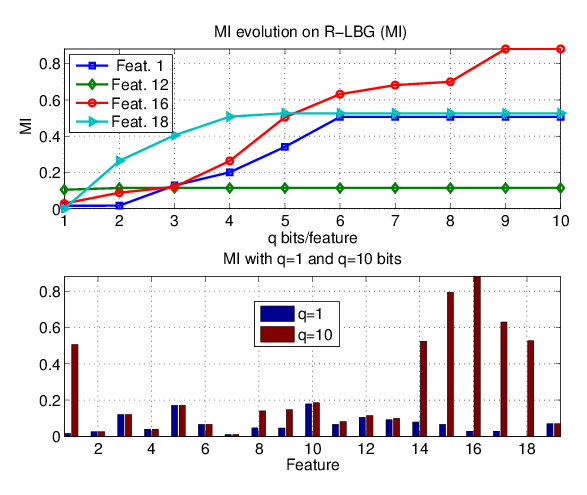
\includegraphics[width=0.6\textwidth]{fig1.png}
\end{figure}
\vspace{-2mm}
{\small Top: MI as
  a function of the number of bits $q \in  \{1,\ldots,10\}$, for features 1,
  12 (which is categorical), 16, and 18.

  Bottom: MI with $q=1$ and $q=10$ bits.}
\end{frame}


% 13
\subsection[Mutual Information Discretization]{Mutual Information Discretization (MID)}
\begin{frame}{Proposal 2: Mutual Information Discretization}
The key motivations for the MID algorithm are as follows:
\begin{itemize}
	\vfill
	\item good FS criteria should also be adequate for FD

	\vfill
	\item MI between features and class labels $\mathbf{y}$ is adequate for FS

  \vfill
	\item the Hellman-Raviv (1970) and Santhi-Vardi (2006) bounds relate the Bayes error
	with the MI
	\begin{equation} \nonumber
	err_{Bayes}( \widetilde{X}_i ) \leq \frac{1}{2} H( \mathbf{y}|\widetilde{X}_i ) \qquad
	err_{Bayes}( \widetilde{X}_i ) \leq 1 - 2^{-H(\mathbf{y} | \widetilde{X}_i  )}.
	\end{equation}
	
  \vfill
	\item Recall that $MI(\widetilde{X}_i;\mathbf{y}) = \underbrace{H(\mathbf{y})}_{\mbox{fixed}} - H(\mathbf{y} | \widetilde{X}_i  )$.
\end{itemize}
\end{frame}


% 14
\begin{frame}{MID: how does it work}
\begin{itemize}
	\item illustration for a given feature ($q=3$ bit)
	\item it computes the cut-points that maximize the MI of the discrete feature with the class label
\end{itemize}
\begin{figure}
	\centering
	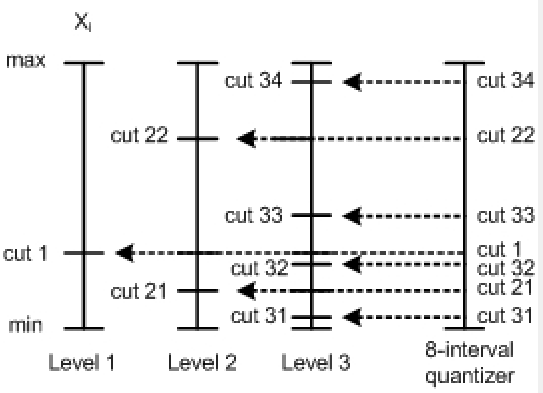
\includegraphics[width=0.5\textwidth]{fig2.png}
\end{figure}
{\small MID is an incremental and recursive partition algorithm}
\end{frame}


% 15
\begin{frame}{MID: fixed and variable versions}
We propose two versions of MID:
\begin{itemize}
	\item MID-fixed, applies MID with $q$ bits per feature
	\item MID-variable, allocates \emph{up to} $q$ bits per feature
\end{itemize}

\vfill
MID-variable is controlled by a
(nonnegative) stopping factor $\epsilon$:
\begin{itemize}
	\vfill
	\item $MI(\widetilde{X}_i^{(b)};\mathbf{y})$ is computed
		
	\vfill
	\item for each feature, discretization is halted at $b$ bits, whenever
	$MI(\widetilde{X}_i^{(b)};\mathbf{y}) - MI(\widetilde{X}_i^{(b-1)};\mathbf{y}) < \epsilon$
	
	\vfill
	\item setting $\epsilon=0$ leads to the minimum number of bits that maximizes the MI
	
	\vfill
	\item for a given $q$, MID-variable will produce
fewer discretization intervals than MID-fixed
\end{itemize}
\end{frame}


% 16
\begin{frame}{MID: evolution of MI}
MI evolution as a function of the number of bits on the Wine dataset ($d=13$ features)
\begin{figure}
	\centering
	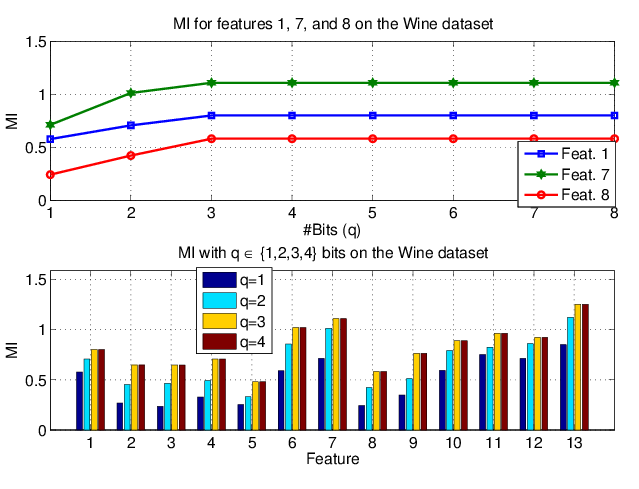
\includegraphics[width=0.65\textwidth]{fig3.png}
\end{figure}
{\small Top: MI for features 1, 7, and 8, with $q \in \{1,\ldots,8\}$.
  Bottom: MI between discretized features and the class label, for $q \in \{1,2,3,4\}$}
\end{frame}


% 17
\section[Experimental Evaluation]{Experimental Evaluation}
\begin{frame}{Experimental Evaluation: Task and Datasets}
\begin{itemize}
	\item Supervised classification with linear SVM, na\"{\i}ve Bayes (NB), and k-nearest neighbors (KNN)
	\item 10-fold cross-validation
	\item UCI, microarray$^\$$, and face images$^\#$ datasets with $d$ features, $c$ classes, and $n$ patterns (in some cases, $d \gg n$)
\end{itemize}
\vfill
\begin{table}
	\centering \scriptsize
	\begin{tabular}{|l|r|r|r||l|r|r|r|}
		\hline
		\textbf{Dataset} & $d$   &  $c$   & $n$    &  \textbf{Dataset} & $d$   &  $c$   & $n$  \\ \hline \hline
 	  Wine             & 13    &   3    &  178   &  Leukemia1$^\$$       & 5327    &   3    & 72 \\ \hline
 		Hepatitis        & 19    &   2    &  155   &  TOX-171$^\$$	 				 & 5748	   &   4	  &  171	\\ \hline
 		Ionosphere       & 34    &   2    &  351   &  Brain-Tumor1$^\$$    & 5920    &   5    &   90   \\ \hline
 		Colon$^\$$           & 2000    &   2    & 62   &  ORL10P$^\#$           & 10304   &  10   &  100    \\ \hline
 		SRBCT$^\$$           & 2309    &   4    & 83   & Prostate-Tumor$^\$$   & 10509   &   2    &  102 \\ \hline
 		AR10P$^\#$          & 2400    &  10    &   130  &   	   Leukemia2$^\$$       & 11225   &   3    &   72   \\ \hline
    PIE10P$^\#$         & 2420    &  10    &   210  &       GLI-85$^\$$	         & 22283	 &   2	  &   85   \\ \hline 		
\end{tabular}
\label{TAB1}
\end{table}
\end{frame}


% 18
\subsection[R-LBG and MID]{R-LBG and MID}
\begin{frame}{Experimental Results: R-LBG and MID 1/3}
\begin{table} [t]
\scriptsize{R-LBG ($@rel=MI$) and \emph{MID-variable} with $q=4$ and linear SVM classifier\\ First row:
total number of bits per instance\\ Second row: test  error rate (\%)} \\ \vspace{2mm}
\label{TAB2} \centering \scriptsize
\begin{tabular}{lr|r|r|r|}
  \cline{2-5}
    & \multicolumn{2}{|c|}{\textbf{R-LBG (MI)}} & \multicolumn{2}{|c|}{\textbf{MID variable}} \\ \hline

   \multicolumn{1}{|c|}{\textbf{Dataset / No FD}} & $\epsilon=0$ & $\epsilon=0.1$ & $\epsilon=0$ & $\epsilon=0.1$  \\ \hline

   \multicolumn{1}{|l|}{Wine} & 52.0 & 30.6 & 38.3  & \textbf{26.2}  \\ \cline{2-5}
   \multicolumn{1}{|l|}{3.9}  & 2.8 & \textbf{1.7}  &  3.4  &  2.8  \\ \hline

   \multicolumn{1}{|l|}{Hepatitis} & 46.5 & 68.8 & \textbf{28.5} & 65.6  \\ \cline{2-5}
   \multicolumn{1}{|l|}{21.3}   & \textbf{15.5} & 21.9  &  18.7  &  18.1  \\ \hline

   \multicolumn{1}{|l|}{Ionosphere} & 129.0 & 102.4 & \textbf{73.0} & 85.0  \\ \cline{2-5}
   \multicolumn{1}{|l|}{12.8}    &  14.0 & 12.5  &  9.4  &  \textbf{5.7}  \\ \hline

   \multicolumn{1}{|l|}{Colon}   & 7954.6 & 7564.0 & \textbf{4682.0} & 6151.9  \\ \cline{2-5}
   \multicolumn{1}{|l|}{17.7}    &  19.4 & \textbf{14.5}  &  19.4  &  \textbf{14.5}  \\ \hline

   \multicolumn{1}{|l|}{SRBCT} & 9222.5 & 8827.7 & \textbf{7144.2}  & 7180.3  \\ \cline{2-5}
   \multicolumn{1}{|l|}{\textbf{0.0}}   &  \textbf{0.0} & \textbf{0.0}  & \textbf{0.0} & \textbf{0.0}    \\ \hline

   \multicolumn{1}{|l|}{AR10P} & 9599.8 & 9583.2 & \textbf{8620.4}  & 8640.4  \\ \cline{2-5}
   \multicolumn{1}{|l|}{0.8}   &  0.8 & 0.8  & \textbf{0.0} & \textbf{0.0}    \\ \hline

   \multicolumn{1}{|l|}{PIE10P} & 9679.9 & 9662.5 & 8550.7  & \textbf{8543.4}  \\ \cline{2-5}
   \multicolumn{1}{|l|}{\textbf{0.0}}   &  \textbf{0.0} & \textbf{0.0}  & \textbf{0.0} & \textbf{0.0}    \\ \hline

\hline
\end{tabular}
\end{table}
\end{frame}


% 19
\begin{frame}{Experimental Results: R-LBG and MID 2/3}
\begin{table} [t]
\scriptsize{R-LBG ($@rel=MI$) and \emph{MID-variable} with $q=4$ and linear SVM classifier\\ First row:
 total number of bits per instance\\ Second row:  test  error rate (\%)} \\ \vspace{2mm}
\label{TAB3} \centering \scriptsize
\begin{tabular}{lr|r|r|r|}
  \cline{2-5}
    & \multicolumn{2}{|c|}{\textbf{R-LBG (MI)}} & \multicolumn{2}{|c|}{\textbf{MID variable}} \\ \hline

   \multicolumn{1}{|c|}{\textbf{Dataset / No FD}} & $\epsilon=0$ & $\epsilon=0.1$ & $\epsilon=0$ & $\epsilon=0.1$  \\ \hline

   \multicolumn{1}{|l|}{Leukemia1} & 21248.2 & 19818.7 & \textbf{14636.9}  & 15555.9  \\ \cline{2-5}
   \multicolumn{1}{|l|}{8.3}   & \textbf{4.2} & 5.6 & 8.3 & 6.9  \\ \hline

   \multicolumn{1}{|l|}{TOX-171} & 22988.5 & 21439.2 & \textbf{19012.4}  & 20070.8  \\ \cline{2-5}
   \multicolumn{1}{|l|}{14.6}   & \textbf{2.3} & 2.9 & 4.1 & 4.1  \\ \hline

   \multicolumn{1}{|l|}{Brain-Tumor1} & 23649.6 & 22174.4 & 17531.0  & \textbf{17436.5}  \\ \cline{2-5}
   \multicolumn{1}{|l|}{11.1}   & \textbf{8.9} & 10.0 & 10.0 & 10.0  \\ \hline

	 \multicolumn{1}{|l|}{ORL10P} & 41215.6 & 41195.1 & 37410.3  & \textbf{37410.2}  \\ \cline{2-5}
   \multicolumn{1}{|l|}{\textbf{1.0}}   & \textbf{1.0} & \textbf{1.0} & 2.0 & 2.0  \\ \hline

	 \multicolumn{1}{|l|}{Prostate-Tumor} & 41735.0 & 40431.3 & \textbf{25493.1}  & 36598.8  \\ \cline{2-5}
   \multicolumn{1}{|l|}{10.8}   & \textbf{7.8} & \textbf{7.8} & \textbf{7.8} & \textbf{7.8}  \\
\hline

	 \multicolumn{1}{|l|}{Leukemia2} & 44300.1 & 40072.9 & 31124.0  & \textbf{30255.4} \\ \cline{2-5}
   \multicolumn{1}{|l|}{5.6}   & \textbf{1.4} & \textbf{1.4} & \textbf{1.4} & \textbf{1.4}  \\
\hline

	\multicolumn{1}{|l|}{GLI-85}  & 88561.7 & 84364.2 & \textbf{54906.9} & 72131.8  \\ \cline{2-5}
\multicolumn{1}{|l|}{10.6}   & \textbf{8.2} & \textbf{8.2} & \textbf{8.2} & \textbf{8.2}  \\
\hline
\end{tabular}
\end{table}
\end{frame}


% 20
\begin{frame}{Experimental Results: R-LBG and MID 3/3}
Some comments on these results:
\begin{itemize}
	\item Obviously, R-LBG with $\epsilon=0$ yields  a larger number of bits per instance, as compared
with $\epsilon=0.1$
	
	\item R-LBG with $\epsilon=0$ attains maximum relevance and better accuracy than with $\epsilon = 0.1$

	\item MID-variable with $\epsilon=0$ yields the
minimum number of bits that ensure the maximum MI

	\item MID-variable with $\epsilon=0$ usually attains
	the better results with a few exceptions
\end{itemize}

\vfill
The Friedman test reported a p-value of $0.04164 < 0.05$
\end{frame}


% 21
\begin{frame}{R-LBG and MID: sensitivity to the $\epsilon$ parameter}
Average bits/instance and test set error rate (\%, NB classifier)
as function of the $\epsilon$ parameter
\begin{figure}
	\centering
	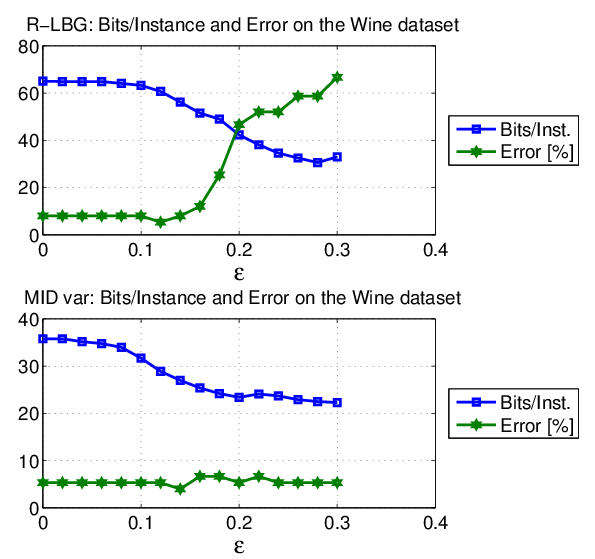
\includegraphics[width=0.6\textwidth]{fig4.png}
\end{figure}
{\small Wine dataset with $q=5$ bits. Top: R-LBG (MI) Bottom: MID-variable}
\end{frame}


% 22
\begin{frame}{R-LBG and MID: sensitivity on the $q$ parameter}
Average bits/instance and test set error rate (\%, NB classifier)
as function of the $q$ parameter
\begin{figure}
	\centering
	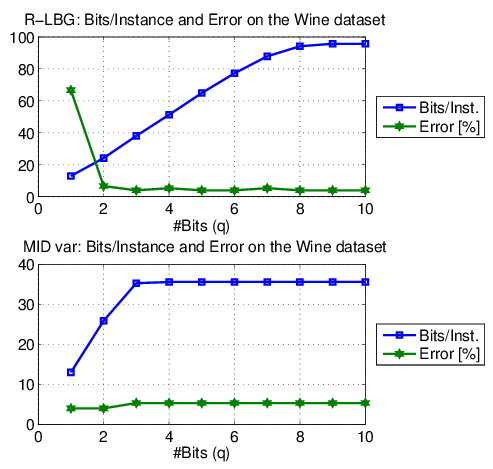
\includegraphics[width=0.6\textwidth]{fig5.png}
\end{figure}
{\small Wine dataset with $\epsilon=0.05$. Top: R-LBG (MI) Bottom: MID-variable}
\end{frame}


% 23
\subsection[Unsupervised FD]{Unsupervised FD}
\begin{frame}{Experimental Results: Unsupervised FD}
\begin{table} [t]
\scriptsize{Unsupervised FD with $q=3$ bit/feature, $@rel=NVAR$,
and $\epsilon=0.25$ \\
First row: total number of bits per instance\\
Second row: test error rate (\%), linear SVM classifier} \\ \vspace{2mm}
\centering \scriptsize
\hspace{-0.4cm}
\scalebox{0.85}{\begin{tabular}{lr|r|r|r|r|r|r|}
  \cline{3-8}
    & & \multicolumn{5}{|c|}{\textbf{Previous methods}} & \multicolumn{1}{|c|}{\textbf{Proposed}} \\ \hline
   \multicolumn{1}{|c|}{{Dataset}} & \multicolumn{1}{|c|}{{No FD}} & \multicolumn{1}{|c|}{\textbf{EIB}} & \multicolumn{1}{|c|}{\textbf{EFB}} & \multicolumn{1}{|c|}{\textbf{PkID}} & \multicolumn{1}{|c|}{\textbf{U-LBG1}} & \multicolumn{1}{|c|}{\textbf{U-LBG2}} & \multicolumn{1}{|c|}{\textbf{R-LBG}}  \\ \hline
 	 \multicolumn{1}{|l|}{AR10P}  &  & 7200.0 & 7200.0 & 9267.8 & 7200.0 & 7200.0 & \textbf{6568.6}  \\ \cline{2-8}
   \multicolumn{1}{|l|}{ }    & 0.8 & \textbf{0.0} & 0.8 & 0.8 & 0.8 & 0.8 & 1.5 \\ \hline

   \multicolumn{1}{|l|}{PIE10P}  &  & 7260.0 & 7260.0 & 9680.0 & 7260.0 & 7260.0 & \textbf{3774.4}  \\ \cline{2-8}
   \multicolumn{1}{|l|}{ }    & \textbf{0.0} & \textbf{0.0} & \textbf{0.0} & \textbf{0.0} & \textbf{0.0} & \textbf{0.0} & \textbf{0.0} \\ \hline

   \multicolumn{1}{|l|}{Leuk.1}  &  & 15981.0 & 15981.0 & 15981.0 & 15981.0 & 15981.0 & \textbf{5733.0} \\ \cline{2-8}
   \multicolumn{1}{|l|}{ }    &  5.6   & \textbf{2.8} & 4.2 & 4.2 & 4.2 & 4.2 & \textbf{2.8} \\ \hline

   \multicolumn{1}{|l|}{TOX-171}  &  & 17244.0 & 17244.0 & 22992.0 & 17244.0 & 17244.0 & \textbf{5847.6} \\ \cline{2-8}
   \multicolumn{1}{|l|}{ }    & 9.9  & \textbf{1.2}     &  1.8    &  \textbf{1.2}    & 1.8 & 1.8 & 8.2  \\ \hline

	 \multicolumn{1}{|l|}{B-Tumor1}  &  & 17760.0 & 17760.0 & 23680.0 & 17760.0 & 17760.0 & \textbf{6085.4}  \\ \cline{2-8}
   \multicolumn{1}{|l|}{ }    & 13.3 & \textbf{8.9} & 11.1 & 11.1 & \textbf{8.9} & \textbf{8.9} & 11.1 \\ \hline

   \multicolumn{1}{|l|}{ORL10P}  &  & 30912.0 &   30912.0 & 41216.0 &  30912.0 & 30912.0 & \textbf{19385.4} \\ \cline{2-8}
   \multicolumn{1}{|l|}{ }    & \textbf{1.0} & \textbf{1.0} & \textbf{1.0} & \textbf{1.0} & \textbf{1.0} & \textbf{1.0} & \textbf{1.0}\\ \hline

	 \multicolumn{1}{|l|}{P-Tumor}  &  & 31527.0 & 31527.0 & 42035.4 & 31520.0 & 31527.0 & \textbf{11394.0}\\ \cline{2-8}
   \multicolumn{1}{|l|}{ }    & 10.8 & \textbf{8.8} & \textbf{8.8} & \textbf{8.8} & \textbf{8.8} & \textbf{8.8} & \textbf{8.8} \\ \hline

	 \multicolumn{1}{|l|}{Leuk.2}  &  & 33675.0 & 33675.0 & 33675.0 &33675.0 &33675.0 & \textbf{12431.4} \\ \cline{2-8}
   \multicolumn{1}{|l|}{ }  & 4.2 & \textbf{2.8} & \textbf{2.8} & \textbf{2.8} & \textbf{2.8} & \textbf{2.8} & 4.2  \\ \hline

   \multicolumn{1}{|l|}{GLI-85}  &  & 66849.0 & 66849.0 & 66849.0 & 66849.0 & 66849.0 & \textbf{25118.7}\\ \cline{2-8}
   \multicolumn{1}{|l|}{ }    & 14.1 & 10.6 & \textbf{8.2} & \textbf{8.2} & 9.4 & 9.4 & \textbf{8.2} \\ \hline
\end{tabular}}
\end{table}
\end{frame}


% 24
\subsection[Unsupervised FD]{Supervised FD}
\begin{frame}{Experimental Results: Supervised FD}
\begin{table} [t]
\scriptsize{Supervised FD with $@rel=MI$ and $\epsilon=0.1$ \\
First row:  total number of bits per instance\\
Second row: test error rate (\%), linear SVM classifier} \\ \vspace{2mm}
\centering \scriptsize
\scalebox{0.85}{\begin{tabular}{l|r|r|r|r|r|r|r|}
   \cline{2-8}
    & \multicolumn{4}{|c|}{\textbf{Previous methods}} & \multicolumn{3}{|c|}{\textbf{Proposed methods}} \\ \hline

   \multicolumn{1}{|c|}{\textbf{Dataset}} & \multicolumn{1}{|c|}{\textbf{IEM}} & \multicolumn{1}{|c|}{\textbf{IEMV}} & \multicolumn{1}{|c|}{\textbf{CAIM}} & \multicolumn{1}{|c|}{\textbf{CACC}} & \multicolumn{1}{|c|}{\textbf{R-LBG}} & \multicolumn{1}{|c|}{\textbf{MIDf}} & \multicolumn{1}{|c|}{\textbf{MIDv}}  \\ \hline

 \multicolumn{1}{|l|}{AR10P}   & 12903.6 & \textbf{7138.4} & 7200.0 & 7200.0 & 7145.6 & 7200.0 & 7266.3 \\ \cline{2-8}
   \multicolumn{1}{|l|}{ }    & 2.3 & 20.0 & 0.8 & \textbf{0.0} & \textbf{0.0} & \textbf{0.0} & \textbf{0.0} \\ \hline

   \multicolumn{1}{|l|}{PIE10P} & 9103.4 & \textbf{5264.0} & 7260.0 & 7260.0 & 7077.3 & 7260.0 & 7154.7 \\ \cline{2-8}
   \multicolumn{1}{|l|}{ }     & \textbf{0.0} & 1.9 & \textbf{0.0} & \textbf{0.0} & \textbf{0.0} & \textbf{0.0} & \textbf{0.0} \\ \hline

   \multicolumn{1}{|l|}{Leuk.1}   & 28435.3 & 26034.7 & * &* & 14656.1 & 15981.0 & \textbf{14278.0} \\ \cline{2-8}
   \multicolumn{1}{|l|}{ }     & 40.3 & 56.9 & * & * & 4.2 & \textbf{2.8} & \textbf{2.8} \\ \hline

   \multicolumn{1}{|l|}{TOX-171}   & 36134.8 & 28253.7 & * & * & \textbf{15725.6} & 17244.0 & 15824.2 \\ \cline{2-8}
   \multicolumn{1}{|l|}{ }     & 5.8 & \textbf{2.9} & * & * & \textbf{2.9} & 3.5 & 4.7  \\ \hline

	 \multicolumn{1}{|l|}{B.-Tumor1}  & 32808.3 & 27133.5 & * & * & \textbf{15674.3} & 17760.0 & 16343.6 \\ \cline{2-8}
   \multicolumn{1}{|l|}{ }     & 20.0 & 35.6 & * & * & 11.1 & 10.0 & \textbf{8.9} \\ \hline

   \multicolumn{1}{|l|}{ORL10P}  & 26475.7 & \textbf{24176.8} & * & * & 30863.0 & 30912.0 & 30786.9\\ \cline{2-8}
   \multicolumn{1}{|l|}{ }     & 9.0 & \textbf{1.0} & * & * & 2.0 & 2.0 & 2.0 \\ \hline

   \multicolumn{1}{|l|}{P.-Tumor}  & 54395.6 & 51964.7 & * & * & 30695.0 & 31527.0 & \textbf{28506.3} \\ \cline{2-8}
   \multicolumn{1}{|l|}{ }    & 12.7  & 11.8 & * & * & \textbf{5.9} & 6.9 & 7.8   \\ \hline

	 \multicolumn{1}{|l|}{Leuk.2}  & 48380.1 & 40447.3 & * & * & 28857.3 & 33675.0 & \textbf{28670.8} \\ \cline{2-8}
   \multicolumn{1}{|l|}{ }     & 8.3 & 6.9 & * & * &  \textbf{2.8} & \textbf{2.8} & \textbf{2.8} \\ \hline

   \multicolumn{1}{|l|}{GLI-85} & 135866.9 & 130689.1 & * & * & 64065.0 & 66849.0 & \textbf{58633.4} \\ \cline{2-8}
   \multicolumn{1}{|l|}{ }     & 11.8 & 12.9 & * & * & \textbf{9.4} & \textbf{9.4} & 10.6 \\ \hline
\end{tabular}}
\end{table}
\end{frame}


% 25
\section[Conclusions]{Conclusions}
\begin{frame}{Conclusions}
Our FD methods (Relevance-LBG and MID):
\begin{itemize}%[<+->]
		\item for both unsupervised and supervised FD, attain equal or better results than state-of-the-art techniques
	  \item scale well for high-dimensional data, contrary to other approaches
	  \item have shown the adequacy of MI between features and class labels for discretization
		\item attain adequate discretizations with a variable number
of bits per feature
\end{itemize}

\vfill
In future work, we will explore the embedding of feature selection
in the discretization process
\end{frame}

\end{document}
